\section{One-Shot 扩展至多教师 OPD}
\label{sec:mopd}

第~\ref{sec:state-diversity} 节表明，一个小型且语义多样的查询集可以在单一领域内达到全数据同策略蒸馏（OPD）的性能。现代后训练流水线通常使用\emph{多教师同策略蒸馏}（MOPD）~\citep{xiao2026mimo,xu2026deepseek}，其中学生模型在单次运行中对多个领域进行训练，每个查询被路由到其对应领域的教师模型。本节探讨的问题是：\textit{相同的查询多样性效果是否依然成立：对于每个领域，一个小型且多样化的查询集能否达到全数据MOPD的性能？}

\begin{tcolorbox}[takeawaysbox]
    每个领域内16个语义多样的查询就足以达到与全数据MOPD相当的性能，其平均验证准确率几乎与分离的全数据OPD相同。
\end{tcolorbox}

\begin{figure}[t]
    \centering
    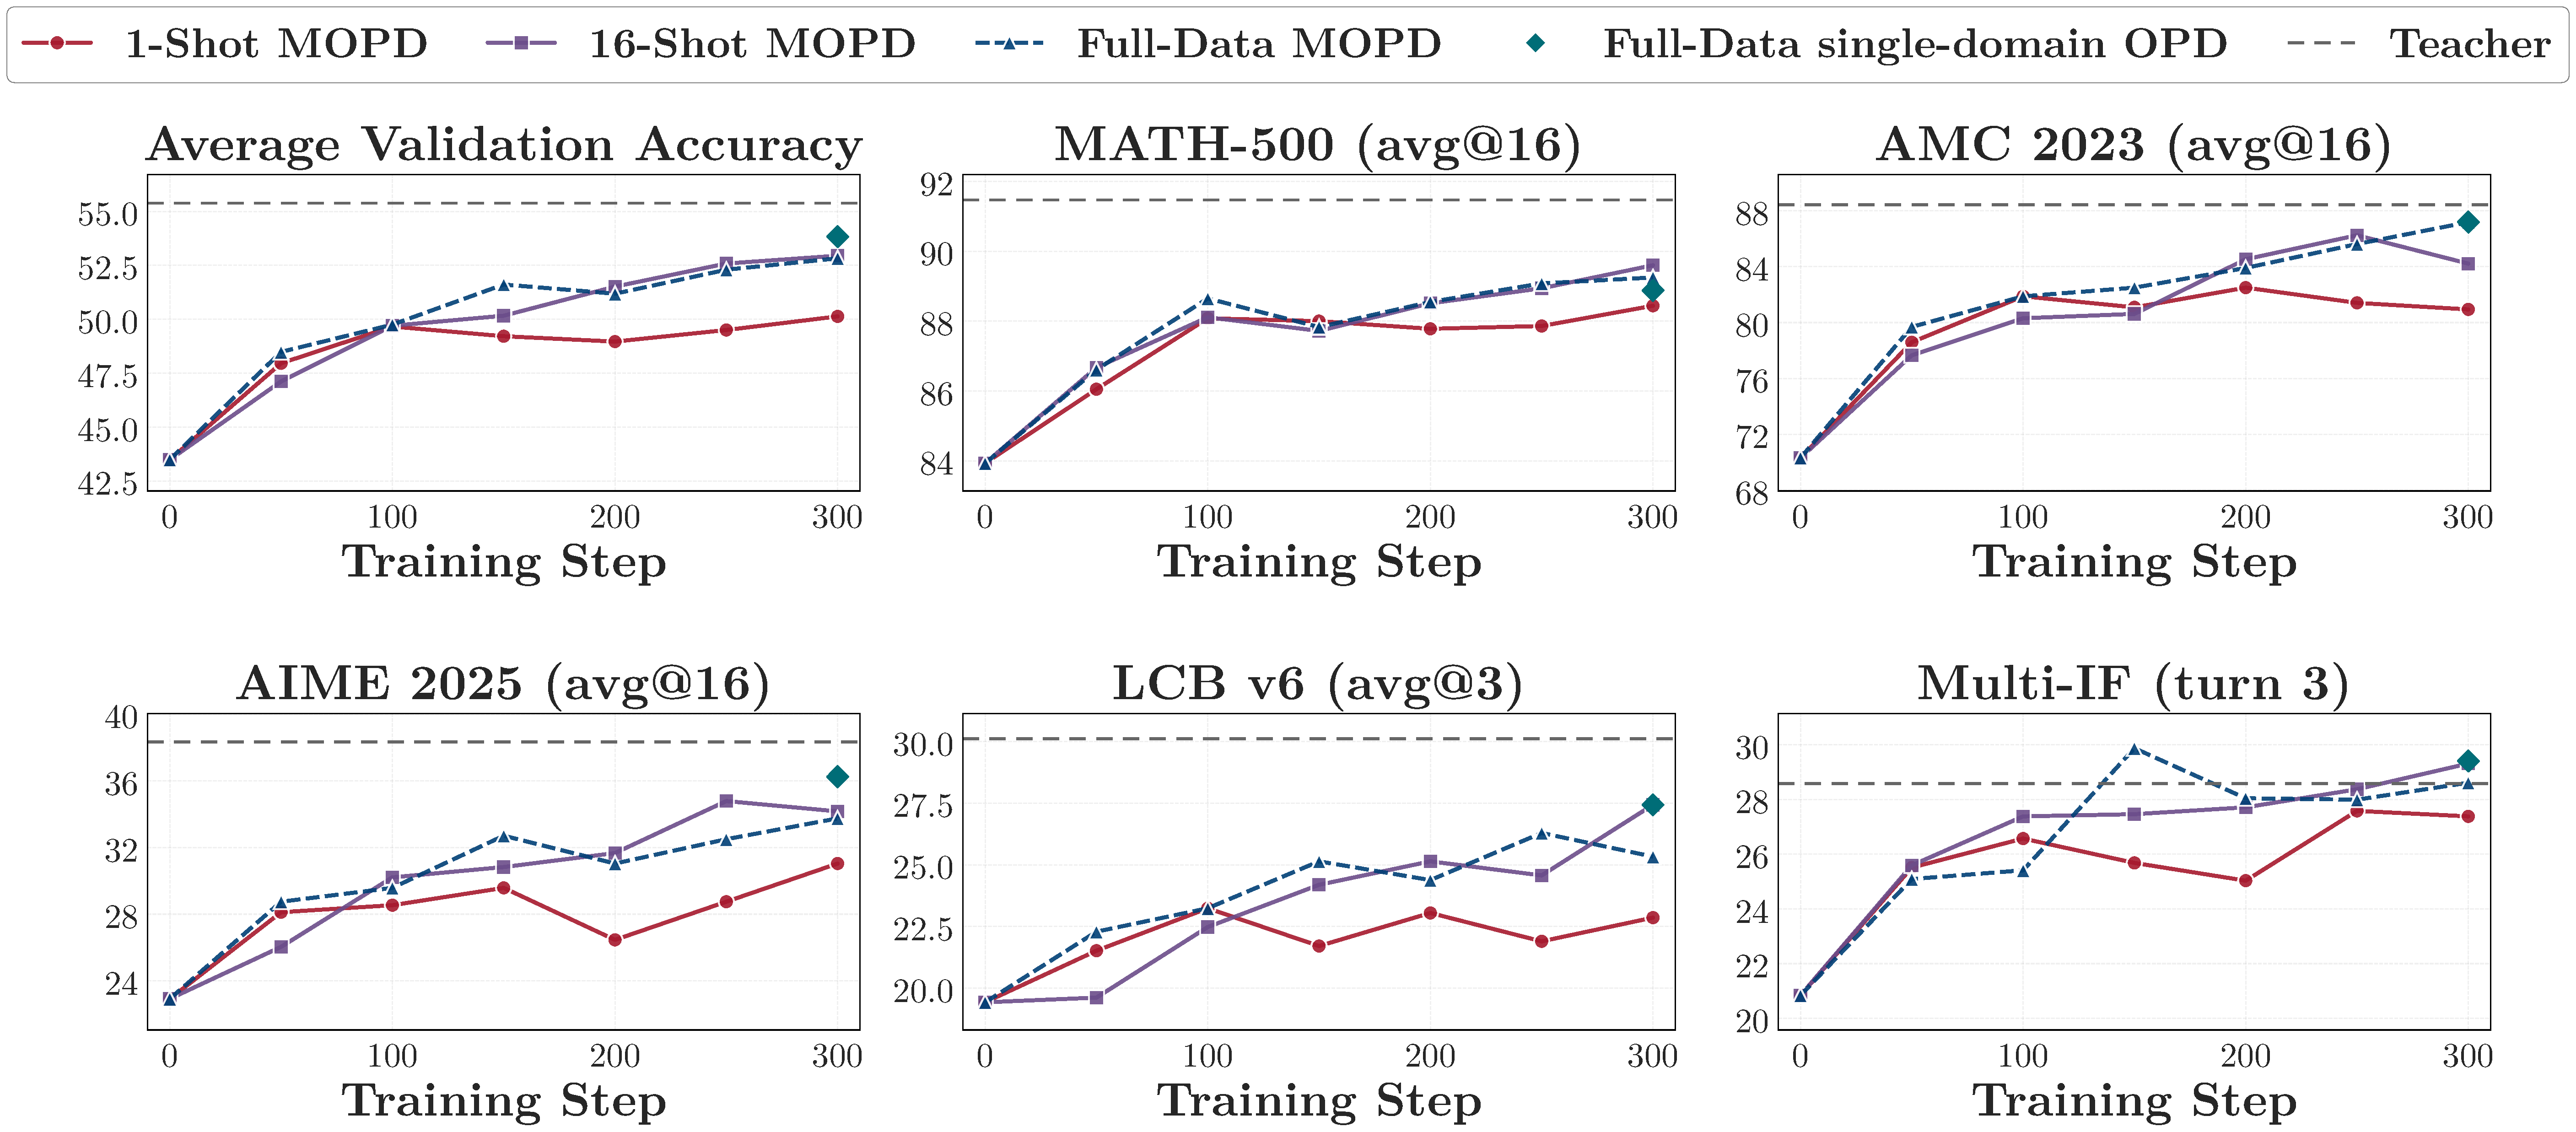
\includegraphics[width=\textwidth]{figures/6_mopd_curves.pdf}
    \caption{
    one-shot、16-shot 和全数据 MOPD 的验证准确率。
    }
    \label{fig:mopd}
\end{figure}

\paragraph{设置}
我们在数学推理、代码生成和指令遵循任务上，使用MOPD训练一个R1-Distill-1.5B学生模型。第\ref{sec:setup}节中的领域教师模型分别为：数学任务使用JustRL-1.5B，代码任务使用Nemotron-1.5B，指令遵循任务使用UltraData-IF-1.5B。我们排除了Agentic工具使用场景，因其采用了一个不同的学生模型Qwen-Coder-1.5B。这三种设置分别为one-shot、16-shot和全量数据MOPD。与第\ref{sec:state-diversity}节一致，16-shot设置从每个领域内分别拟合的16个BGE-M3~\citep{chen2024bge}语义簇中各选取一个代表性样本。所有设置均运行\(300\)步，所用超参数见表~\ref{tab:mopd-hyperparams}。

\paragraph{全数据MOPD与分离的全数据OPD相匹配。}
在步骤 \(300\) 时，全数据 MOPD 将平均验证准确率从 \(43.5\) 提升至 \(52.8\) ，恢复了教师-学生差距的 \(79\%\) 。三个对应的全数据 OPD 运行分别达到 \(53.8\) 。这一 \(1.0\) 点的差异表明，当三个领域在单次运行中同时训练时，MOPD 依然有效，并确立了全数据 MOPD 作为下文查询多样性比较的基准。

\paragraph{每个领域16个多样化查询即可匹配全数据MOPD。}
将每个领域的查询数量从1增加到16，使平均验证准确率在步骤\(300\)时从\(50.1\)提升至\(52.9\)。全数据MOPD达到\(52.8\)，因此16次查询MOPD恢复了全数据MOPD增益的\(101\%\)。该结果并非由单一领域驱动：分别计算，对应的比例分别为数学领域的\(93\%\)、代码生成领域的\(136\%\)以及指令遵循领域的\(109\%\)。由于16次查询和全数据MOPD使用相同的回滚和最优化预算，因此在此情景下，将每个领域的查询集扩展到超过16个多样化查询不会带来额外的平均增益。

这些结果共同支持了MOPD的状态空间解释：语义多样的查询可以在每个领域内引发互补状态，使得每个领域16个查询即可达到全数据MOPD的效果。


